% ============================================================
%  MCD101 – Programación en Ciencia de Datos
%  Informe Final – Formato IEEE
%  Dataset: Bank Marketing (UCI Repository)
% ============================================================
\documentclass[conference]{IEEEtran}

% ── Paquetes ────────────────────────────────────────────────
\usepackage[utf8]{inputenc}
\usepackage[T1]{fontenc}
\usepackage[spanish]{babel}
\usepackage{cite}
\usepackage{amsmath,amssymb}
\usepackage{graphicx}
\usepackage{booktabs}
\usepackage{array}
\usepackage{url}
\usepackage{hyperref}
\usepackage{xcolor}
\usepackage{float}
\usepackage{multirow}
\usepackage{siunitx}

% ── Configuración de hyperref ────────────────────────────────
\hypersetup{
    colorlinks = true,
    linkcolor  = blue,
    citecolor  = blue,
    urlcolor   = blue
}

% ============================================================
\begin{document}

% ── Título y autores ─────────────────────────────────────────
\title{Análisis Exploratorio y Estadística Descriptiva del Conjunto de Datos Bank Marketing para la Predicción de Suscripción Bancaria}

\author{
    \IEEEauthorblockN{Fabrizio Roy Choque Ormachea}
    \IEEEauthorblockA{
        \textit{Maestría en Ciencia de Datos}\\
        \textit{Universidad Nacional del Altiplano Puno}\\
        Puno, Perú\\
        20181167@lamolina.edu.pe
    }
    \and
    \IEEEauthorblockN{Milton Hiroshi Taco Aviles}
    \IEEEauthorblockA{
        \textit{Maestría en Ciencia de Datos}\\
        \textit{Universidad Nacional del Altiplano Puno}\\
        Puno, Perú\\
        htacoav@gmail.com
    }
}

\maketitle

% ── Resumen ──────────────────────────────────────────────────
\begin{abstract}
Este trabajo presenta un análisis exploratorio exhaustivo del conjunto de datos \textit{Bank Marketing} del repositorio UCI, recopilado a partir de campañas de marketing telefónico realizadas por una institución bancaria portuguesa. El estudio se centra en caracterizar estadísticamente las 16 variables del conjunto de datos, identificar patrones relevantes, tratar valores faltantes implícitos y visualizar la relación entre las características y la variable objetivo: la suscripción de un depósito a plazo fijo. Se analizan distribuciones, medidas de tendencia central y dispersión, asimetría, curtosis y valores atípicos para las variables numéricas, así como frecuencias y tasas de suscripción para las variables categóricas. Como aplicación del análisis exploratorio, se entrenan dos modelos de clasificación supervisada —Regresión Logística y Random Forest— bajo configuraciones con y sin la variable \texttt{duration}, validando que las características identificadas durante la exploración efectivamente contribuyen a la predicción. Los hallazgos muestran que variables como \texttt{poutcome}, \texttt{month}, \texttt{job} y \texttt{balance} son los predictores más informativos en un escenario accionable.
\end{abstract}

\begin{IEEEkeywords}
análisis exploratorio de datos, estadística descriptiva, marketing bancario, visualización de datos, clasificación binaria, Random Forest, ciencia de datos
\end{IEEEkeywords}

% ============================================================
\section{Introducción}

El análisis exploratorio de datos (EDA, por sus siglas en inglés) constituye una etapa fundamental en cualquier proyecto de ciencia de datos. Antes de construir cualquier modelo predictivo, comprender la estructura, distribución y relaciones entre las variables del conjunto de datos permite tomar decisiones informadas sobre el preprocesamiento, la selección de características y la elección de algoritmos \cite{tukey1977}.

El conjunto de datos \textit{Bank Marketing} \cite{uci_bank}, recopilado de campañas de marketing telefónico de un banco portugués entre 2008 y 2013, representa un caso de estudio rico y desafiante: presenta desbalance de clases, variables categóricas con valores desconocidos, y una mezcla de características demográficas, financieras y de campaña. Estas características lo convierten en un escenario ideal para ilustrar técnicas de exploración y análisis estadístico aplicadas a problemas reales.

El problema de predicción subyacente —determinar si un cliente suscribirá un depósito a plazo fijo— es secundario al análisis exploratorio en este trabajo, y sirve principalmente como marco de validación para los patrones identificados durante la exploración.

\subsection*{Objetivo del estudio}

Realizar un análisis exploratorio completo del conjunto de datos \textit{Bank Marketing}, caracterizando estadísticamente sus variables, identificando patrones y relaciones relevantes mediante visualizaciones, y validando los hallazgos a través de modelos de clasificación supervisada.

\subsection*{Organización del informe}

La Sección~\ref{sec:arte} revisa trabajos relacionados. La Sección~\ref{sec:datos} constituye el núcleo del trabajo, con la descripción y análisis estadístico completo del conjunto de datos. La Sección~\ref{sec:metodo} describe brevemente la metodología de modelado. La Sección~\ref{sec:resultados} presenta los resultados de los modelos como validación de los hallazgos exploratorios. La Sección~\ref{sec:conclusiones} expone las conclusiones y trabajos futuros.

% ============================================================
\section{Estado del Arte}
\label{sec:arte}

\subsection{Análisis exploratorio en conjuntos de datos de marketing}

El análisis exploratorio de datos en el contexto del marketing bancario ha sido señalado como una etapa crítica para entender el comportamiento del cliente. Moro et al.\ \cite{moro2014} demostraron que una cuidadosa selección de características basada en el análisis previo de importancia de variables permitió reducir el número de contactos necesarios en una campaña manteniendo altas tasas de éxito, subrayando el valor del EDA antes del modelado.

Chapman et al.\ \cite{crisp2000} propusieron la metodología CRISP-DM, ampliamente adoptada en la industria, en la que el entendimiento y la exploración de los datos ocupan dos de las seis fases principales del proceso, evidenciando su centralidad en cualquier proyecto de ciencia de datos.

\subsection{Trabajos que utilizan el conjunto de datos Bank Marketing}

El conjunto de datos \textit{Bank Marketing} es uno de los más referenciados en el repositorio UCI \cite{uci_bank}. Ha sido ampliamente utilizado para comparar algoritmos de clasificación \cite{bhatt2020}, estudiar el efecto del desbalance de clases, y como caso de uso en técnicas de explicabilidad como SHAP y LIME \cite{molnar2020}. Estudios anteriores reportan ROC-AUC entre 0.75 y 0.93 dependiendo del conjunto de características utilizado, siendo los modelos de ensamble los que obtienen consistentemente mejores resultados \cite{ferreira2020}.

% ============================================================
\section{Descripción y Análisis del Conjunto de Datos}
\label{sec:datos}

\subsection{Fuente y características generales}

El conjunto de datos fue obtenido del repositorio UCI Machine Learning Repository \cite{uci_bank}. Contiene \textbf{45{,}211 registros} y \textbf{17 variables}: 16 características de entrada y 1 variable objetivo (\texttt{y}), sin valores nulos explícitos.

\subsection{Número y tipo de características}

Las variables se clasifican según su naturaleza en tres grupos, como se muestra en la Tabla~\ref{tab:variables}.

\begin{table}[H]
\caption{Clasificación de variables del dataset}
\label{tab:variables}
\centering
\begin{tabular}{@{}llp{3.6cm}@{}}
\toprule
\textbf{Tipo} & \textbf{N} & \textbf{Variables} \\
\midrule
Numéricas continuas   & 5 & \texttt{age}, \texttt{balance}, \texttt{duration}, \texttt{campaign}, \texttt{pdays} \\
Numéricas discretas   & 2 & \texttt{previous}, \texttt{day} \\
Categóricas nominales & 9 & \texttt{job}, \texttt{marital}, \texttt{education}, \texttt{default}, \texttt{housing}, \texttt{loan}, \texttt{contact}, \texttt{month}, \texttt{poutcome} \\
Objetivo (binaria)    & 1 & \texttt{y} (\textit{yes/no}) \\
\bottomrule
\end{tabular}
\end{table}

\subsection{Estadística descriptiva de variables numéricas}

La Tabla~\ref{tab:estadistica} resume las principales medidas estadísticas. Se incluyen medidas de posición (media, mediana), dispersión (desviación estándar, mínimo, máximo) y forma (asimetría y curtosis).

\begin{table}[H]
\caption{Estadística descriptiva extendida de variables numéricas}
\label{tab:estadistica}
\centering
\resizebox{\columnwidth}{!}{%
\begin{tabular}{@{}lrrrrrrr@{}}
\toprule
\textbf{Variable} & \textbf{Media} & \textbf{Mediana} & \textbf{D.E.} & \textbf{Mín.} & \textbf{Máx.} & \textbf{Asim.} & \textbf{Curt.} \\
\midrule
\texttt{age}      & 40.9  & 39.0  & 10.6  & 18    & 95     & 0.68  & 0.49 \\
\texttt{balance}  & 1362  & 448   & 3044  & -8019 & 102127 & 5.86  & 66.0 \\
\texttt{duration} & 258.2 & 180.0 & 257.5 & 0     & 4918   & 3.16  & 16.9 \\
\texttt{campaign} & 2.76  & 2.0   & 3.10  & 1     & 63     & 4.76  & 34.8 \\
\texttt{pdays}    & 40.2  & $-1$  & 100.1 & $-1$  & 871    & 3.64  & 13.9 \\
\texttt{previous} & 0.58  & 0.0   & 2.30  & 0     & 275    & 18.3  & 581  \\
\texttt{day}      & 15.8  & 16.0  & 8.32  & 1     & 31     & 0.09  & -1.0 \\
\bottomrule
\multicolumn{8}{l}{\footnotesize D.E. = Desviación Estándar; Asim. = Asimetría; Curt. = Curtosis.}
\end{tabular}%
}
\end{table}

Se destacan los siguientes hallazgos:

\begin{itemize}
    \item \textbf{\texttt{balance}}: presenta la mayor asimetría positiva (5.86) y curtosis extrema (66.0), indicando la presencia de clientes con saldos muy elevados. La mediana (\$448) es muy inferior a la media (\$1{,}362), confirmando este sesgo.
    \item \textbf{\texttt{duration}}: alta asimetría positiva (3.16); la mayoría de llamadas son breves (mediana 180 s), pero existen casos extremos de hasta 4{,}918 segundos (\textasciitilde{}82 minutos).
    \item \textbf{\texttt{campaign}}: el número de contactos por campaña tiene mediana 2, pero puede llegar a 63, sugiriendo estrategias de contacto muy persistentes con algunos clientes.
    \item \textbf{\texttt{pdays}}: toma el valor $-1$ cuando el cliente no fue contactado previamente (81.7\% de los casos), lo que distorsiona la media y requiere tratamiento especial.
    \item \textbf{\texttt{previous}}: altísima asimetría (18.3) y curtosis (581), producto de que la gran mayoría de clientes no había sido contactado antes.
    \item \textbf{\texttt{day}}: distribución aproximadamente uniforme (curtosis $-1.0$), indicando que los contactos se distribuyeron homogéneamente a lo largo del mes.
\end{itemize}

\subsection{Detección de valores atípicos}

Se aplicó el criterio del Rango Intercuartílico (IQR) para identificar valores atípicos. Un valor se considera atípico si cae por debajo de $Q_1 - 1.5 \cdot \text{IQR}$ o por encima de $Q_3 + 1.5 \cdot \text{IQR}$. Los resultados se muestran en la Tabla~\ref{tab:outliers}.

\begin{table}[H]
\caption{Detección de valores atípicos (criterio IQR)}
\label{tab:outliers}
\centering
\resizebox{\columnwidth}{!}{%
\begin{tabular}{@{}lrrlr@{}}
\toprule
\textbf{Variable} & \textbf{Outliers} & \textbf{\%} & \textbf{Lím. inf.} & \textbf{Lím. sup.} \\
\midrule
\texttt{age}      & 280    & 0.62  & 9.5      & 71.5   \\
\texttt{balance}  & 3\,414 & 7.55  & $-$3313  & 5385   \\
\texttt{duration} & 2\,597 & 5.75  & $-$446   & 847    \\
\texttt{campaign} & 2\,396 & 5.30  & $-$3$^\dagger$ & 7 \\
\texttt{pdays}    & 8\,257 & 18.3  & $-$1     & $-$1   \\
\texttt{previous} & 2\,394 & 5.30  & $-$1$^\dagger$ & 1  \\
\texttt{day}      & 0      & 0.00  & $-$9.5$^\dagger$ & 40.5 \\
\bottomrule
\multicolumn{5}{l}{\footnotesize $^\dagger$ El límite negativo no aplica por definición de la variable.}
\end{tabular}%
}
\end{table}

\texttt{balance} concentra el mayor porcentaje de outliers reales (7.55\%), correspondientes a clientes con saldos muy elevados. Para \texttt{pdays}, el alto porcentaje se debe a que el valor $-1$ queda fuera del rango IQR por ser una codificación especial, no un valor atípico real.

 \begin{figure}[H]
    \centering
    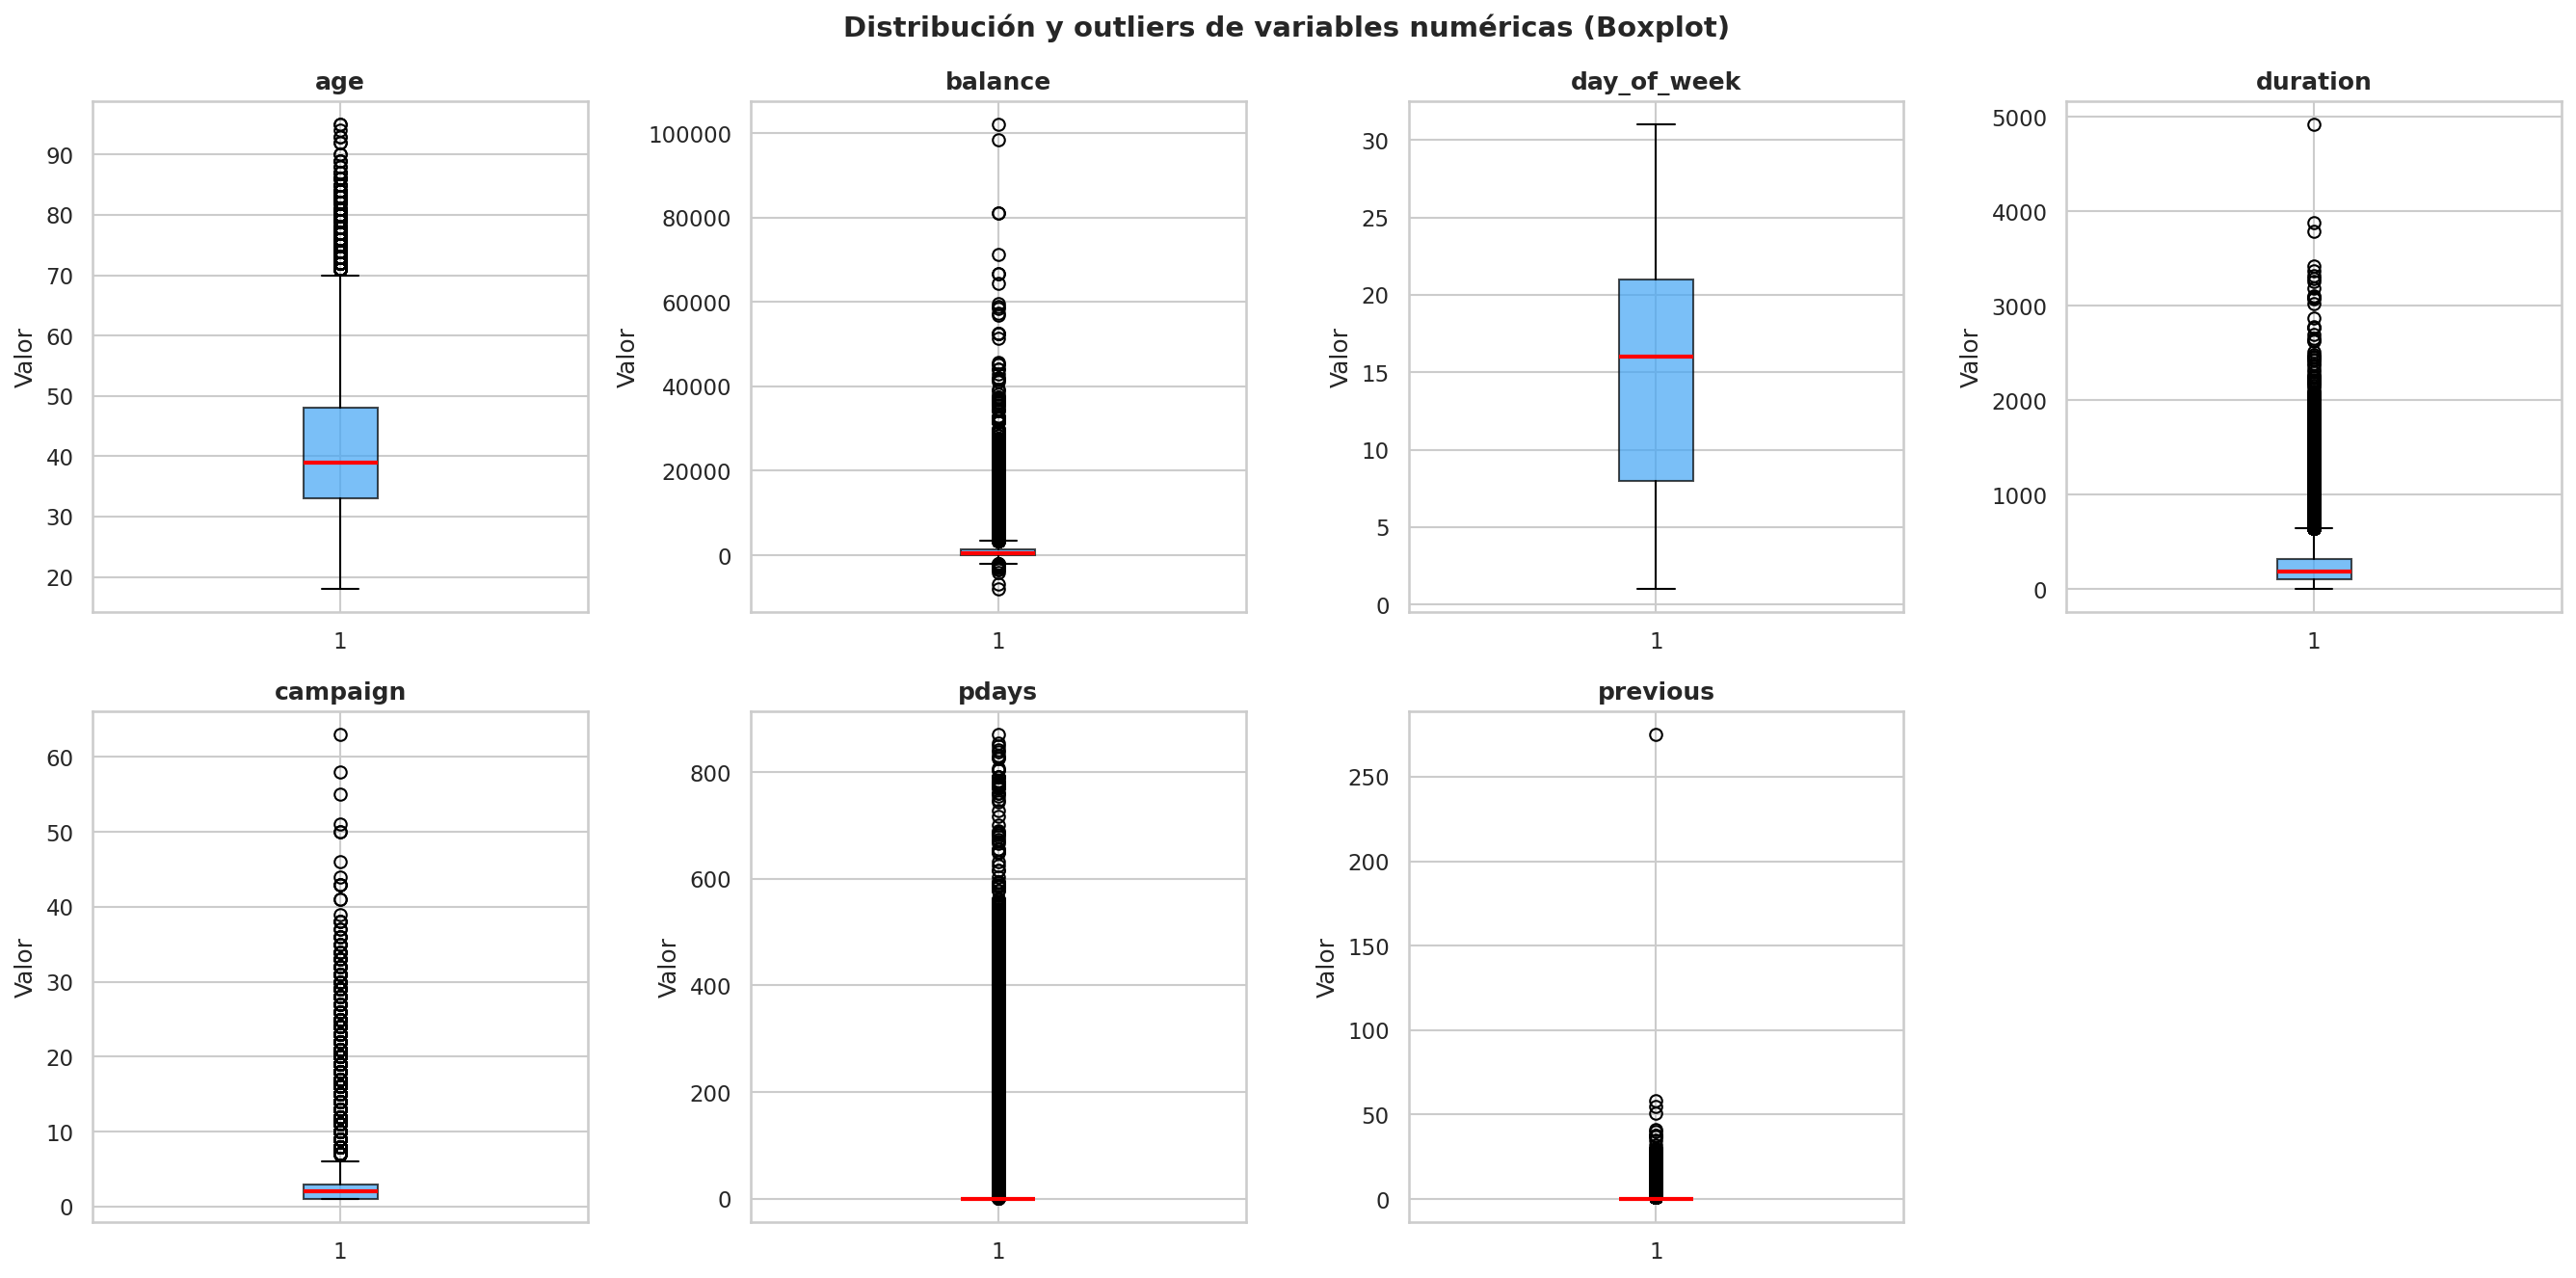
\includegraphics[width=0.95\columnwidth]{boxplots_numericas.png}
    \caption{Boxplots de variables numéricas. Se aprecian los valores atípicos en \texttt{balance}, \texttt{duration} y \texttt{campaign}.}
    \label{fig:boxplots}
 \end{figure}

\subsection{Distribución de la variable objetivo}

El conjunto de datos presenta un marcado \textbf{desbalance de clases}: el 88.3\% de los registros corresponde a clientes que no suscribieron (\textit{no}) y el 11.7\% a quienes sí lo hicieron (\textit{yes}). Este desbalance es representativo de situaciones reales en marketing directo y tiene implicaciones directas en la elección de métricas de evaluación.

\subsection{Análisis de variables categóricas}

La Tabla~\ref{tab:categoricas} resume las frecuencias y tasas de suscripción de las variables categóricas más relevantes.

\begin{table}[H]
\caption{Tasa de suscripción por categorías seleccionadas}
\label{tab:categoricas}
\centering
\resizebox{\columnwidth}{!}{%
\begin{tabular}{@{}llrr@{}}
\toprule
\textbf{Variable} & \textbf{Categoría} & \textbf{Frecuencia (\%)} & \textbf{Tasa suscrip. (\%)} \\
\midrule
\multirow{4}{*}{\texttt{job}}
  & blue-collar & 21.5 & 7.2  \\
  & management  & 20.9 & 13.5 \\
  & technician  & 16.8 & 10.5 \\
  & student     & 2.3  & 28.7 \\
\midrule
\multirow{3}{*}{\texttt{education}}
  & secondary   & 51.6 & 10.5 \\
  & tertiary    & 29.9 & 15.5 \\
  & primary     & 15.2 & 7.2  \\
\midrule
\multirow{3}{*}{\texttt{poutcome}}
  & success     & 3.4  & 64.7 \\
  & failure     & 10.8 & 13.0 \\
  & other       & 4.0  & 16.5 \\
\midrule
\multirow{4}{*}{\texttt{month}}
  & mar         & 1.3  & 51.4 \\
  & sep         & 2.1  & 44.6 \\
  & oct         & 1.8  & 43.5 \\
  & may         & 26.9 & 8.0  \\
\bottomrule
\end{tabular}%
}
\end{table}

Los hallazgos más relevantes son:

\begin{itemize}
    \item \textbf{\texttt{poutcome = success}}: clientes con campaña previa exitosa presentan una tasa de suscripción del 64.7\%, muy superior a la media del 11.7\%. Es el predictor categórico más potente.
    \item \textbf{\texttt{job = student}}: los estudiantes tienen una tasa de suscripción del 28.7\%, casi el triple de la media, posiblemente relacionado con incentivos de ahorro para jóvenes.
    \item \textbf{\texttt{month}}: los meses de marzo, septiembre y octubre presentan tasas superiores al 40\%, mientras que mayo —el mes con más contactos (26.9\%)— tiene solo un 8.0\%. Esto sugiere que la calidad del momento de contacto supera a la cantidad.
    \item \textbf{\texttt{education = tertiary}}: clientes con educación universitaria tienen mayor tasa de suscripción (15.5\%) respecto a los de educación primaria (7.2\%).
\end{itemize}

 \begin{figure}[H]
     \centering
     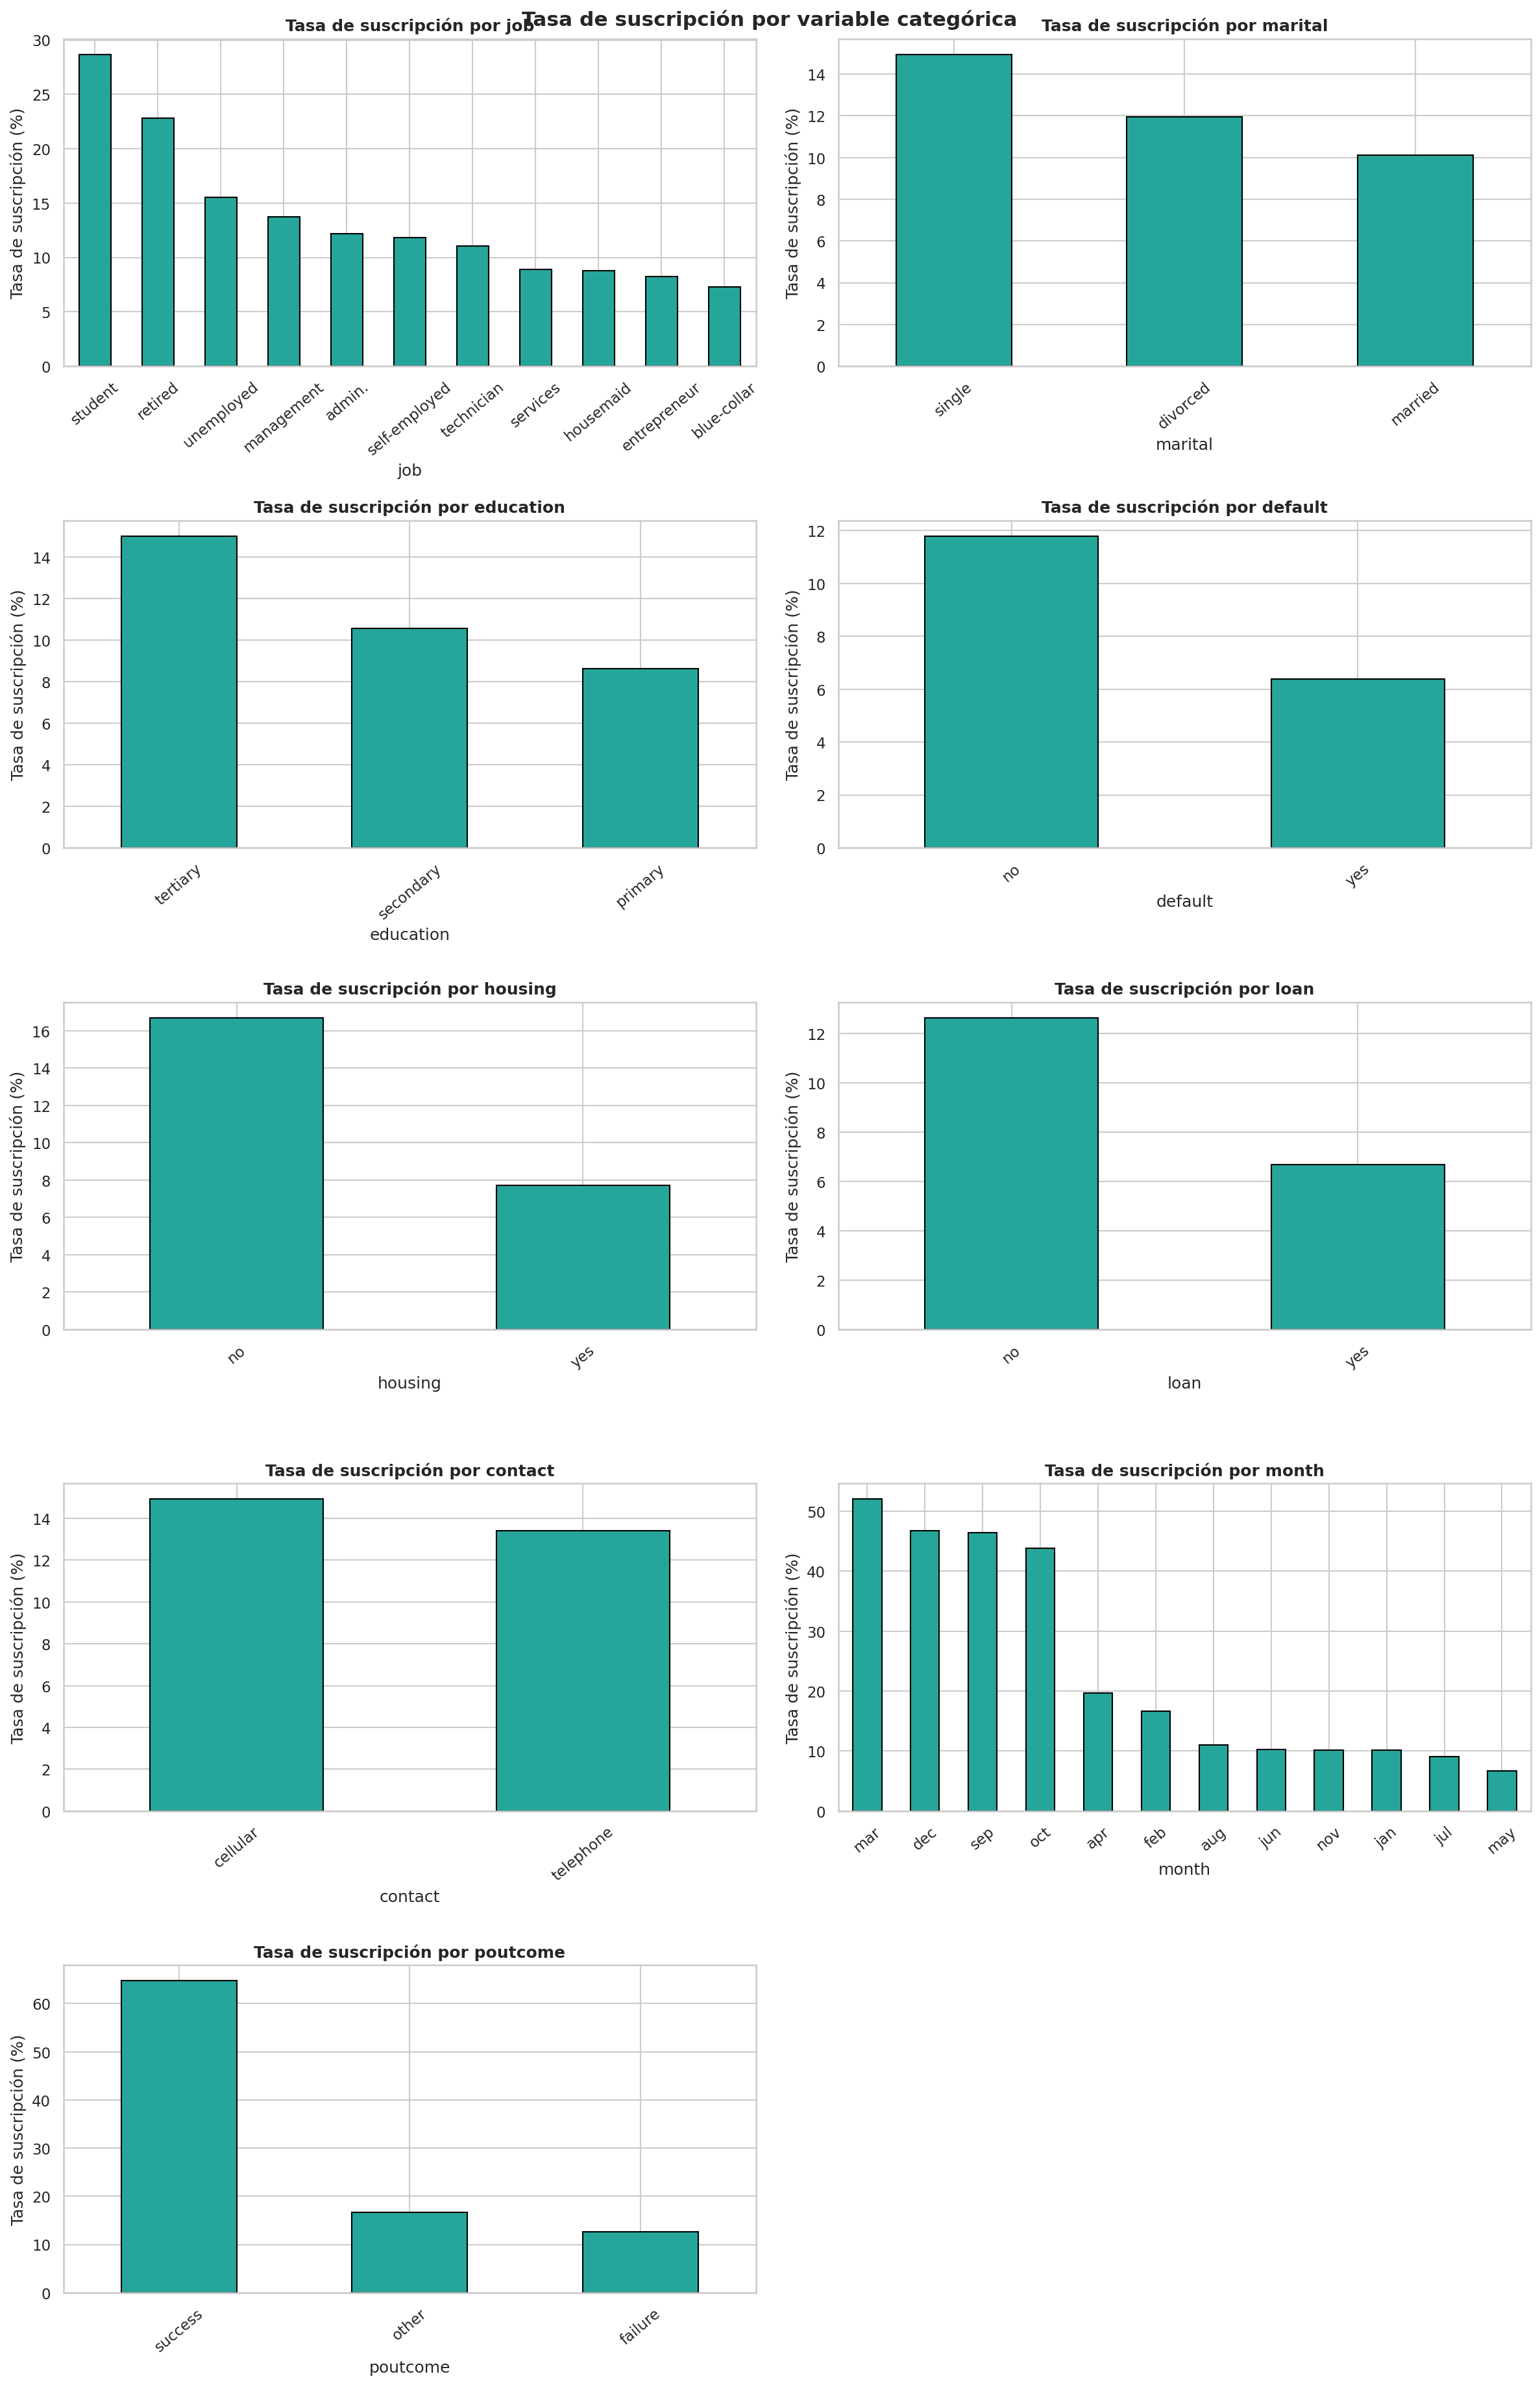
\includegraphics[width=0.95\columnwidth]{tasa_por_categorica.png}
     \caption{Tasa de suscripción por variable categórica.}
     \label{fig:tasa_cat}
 \end{figure}

\subsection{Manejo de datos faltantes implícitos}

El dataset no presenta valores \texttt{NaN}, pero tres variables categóricas contienen la categoría \texttt{'unknown'} como valor faltante implícito (Tabla~\ref{tab:unknown}).

\begin{table}[H]
\caption{Variables con valor \texttt{'unknown'}}
\label{tab:unknown}
\centering
\begin{tabular}{@{}lrr@{}}
\toprule
\textbf{Variable} & \textbf{Registros} & \textbf{Porcentaje} \\
\midrule
\texttt{education} & 1\,857  & 4.11\%  \\
\texttt{contact}   & 13\,020 & 28.79\% \\
\texttt{poutcome}  & 36\,959 & 81.75\% \\
\bottomrule
\end{tabular}
\end{table}

La estrategia adoptada fue \textbf{reemplazar \texttt{'unknown'} por la moda} de cada variable. Para \texttt{poutcome}, el alto porcentaje (81.75\%) se explica porque la mayoría de clientes no participó en campañas anteriores, por lo que este valor refleja información real y no ausencia de dato.

\subsection{Selección de características}

Se calculó la correlación de Pearson entre las variables numéricas y la variable objetivo binarizada. Los resultados se muestran en la Tabla~\ref{tab:correlacion}.

\begin{table}[H]
\caption{Correlación de variables numéricas con la variable objetivo}
\label{tab:correlacion}
\centering
\begin{tabular}{@{}lr@{}}
\toprule
\textbf{Variable} & \textbf{Correlación con \texttt{y}} \\
\midrule
\texttt{duration}  & \phantom{$-$}0.395 \\
\texttt{pdays}     & \phantom{$-$}0.103 \\
\texttt{previous}  & \phantom{$-$}0.083 \\
\texttt{balance}   & \phantom{$-$}0.052 \\
\texttt{day}       & \phantom{$-$}0.030 \\
\texttt{age}       & \phantom{$-$}0.030 \\
\texttt{campaign}  & $-$0.073           \\
\bottomrule
\end{tabular}
\end{table}

\texttt{duration} destaca con correlación de 0.395, sin embargo, es una variable \textbf{no accionable}: su valor se conoce solo al finalizar la llamada, por lo que no puede usarse para decidir a priori a quién contactar. Por este motivo se diseñaron dos experimentos: uno con \texttt{duration} (\textit{benchmark}) y uno sin ella (escenario accionable).

 \begin{figure}[H]
     \centering
     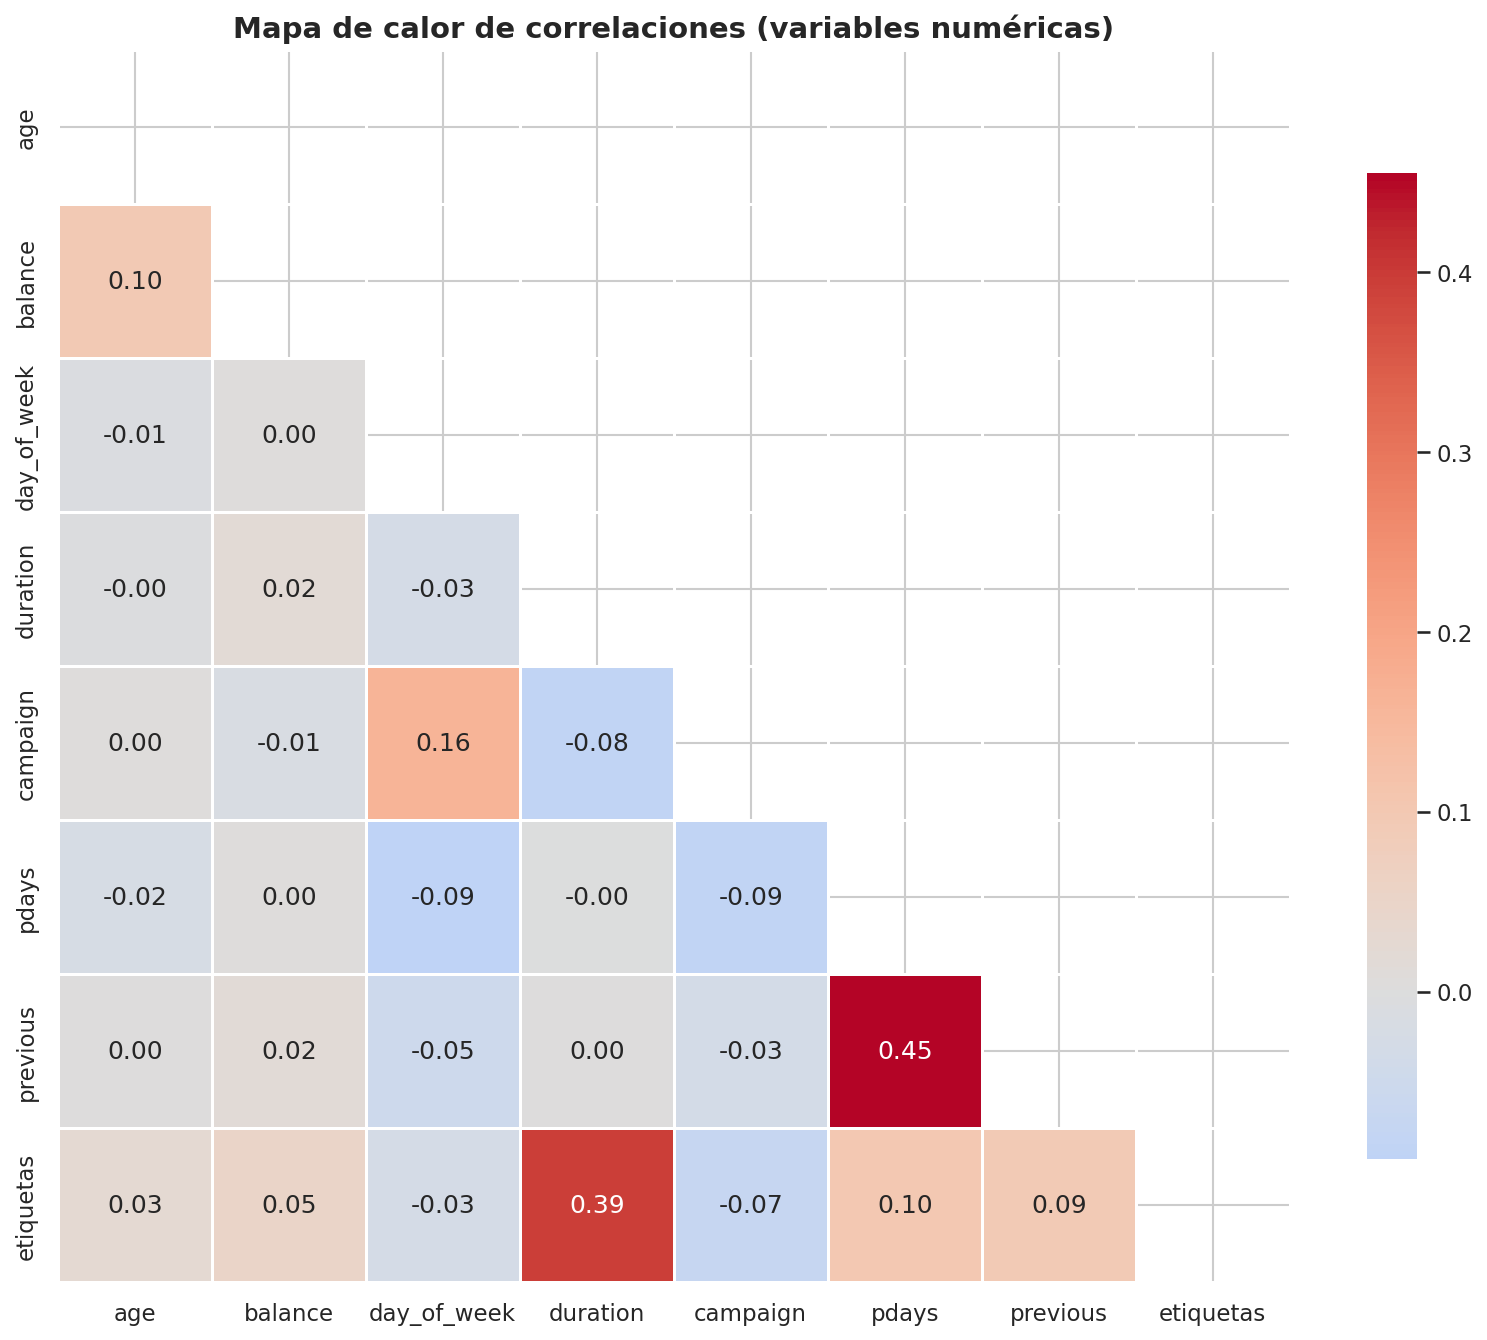
\includegraphics[width=0.95\columnwidth]{heatmap_correlacion.png}
     \caption{Mapa de calor de correlaciones entre variables numéricas y la variable objetivo.}
     \label{fig:heatmap}
 \end{figure}

% ============================================================
\section{Metodología de Modelado}
\label{sec:metodo}

Como validación de los patrones identificados en el análisis exploratorio, se entrenaron modelos de clasificación supervisada. El preprocesamiento consistió en escalado estándar para variables numéricas y codificación one-hot para variables categóricas, implementados en un \textit{pipeline} de scikit-learn. Los datos se dividieron en entrenamiento (60\%), validación (20\%) y prueba (20\%), con estratificación por clase. Se evaluaron dos modelos: \textbf{Regresión Logística} (con pesos balanceados) y \textbf{Random Forest} (250 árboles, pesos balanceados). El umbral óptimo se seleccionó maximizando el F1-score en validación. Dado el desbalance de clases, el \textbf{PR-AUC} fue la métrica principal de comparación.

% ============================================================
\section{Resultados}
\label{sec:resultados}

\subsection{Desempeño de los modelos}

La Tabla~\ref{tab:resultados} resume el desempeño de los modelos, confirmando que las variables identificadas como relevantes durante el análisis exploratorio efectivamente contribuyen a la predicción.

\begin{table}[H]
\caption{Resultados en el conjunto de prueba}
\label{tab:resultados}
\centering
\resizebox{\columnwidth}{!}{%
\begin{tabular}{@{}llccccc@{}}
\toprule
\textbf{Experimento} & \textbf{Modelo} & \textbf{F1} & \textbf{Recall} & \textbf{Precisión} & \textbf{ROC-AUC} & \textbf{PR-AUC} \\
\midrule
Con \texttt{duration} & Random Forest  & 0.608 & 0.734 & 0.519 & 0.925 & 0.607 \\
Con \texttt{duration} & Reg. Logística & 0.579 & 0.721 & 0.484 & 0.907 & 0.536 \\
Sin \texttt{duration} & Random Forest  & 0.480 & 0.507 & 0.457 & 0.799 & 0.448 \\
Sin \texttt{duration} & Reg. Logística & 0.441 & 0.453 & 0.430 & 0.771 & 0.408 \\
\bottomrule
\end{tabular}%
}
\end{table}

\subsection{Curvas ROC y Precisión-Recall}

Las curvas ROC y Precisión-Recall confirman visualmente las diferencias entre modelos. En el escenario accionable (sin \texttt{duration}), el Random Forest obtiene mayor PR-AUC, validando que las características exploradas son informativas incluso sin la variable más correlacionada.

 \begin{figure}[H]
     \centering
     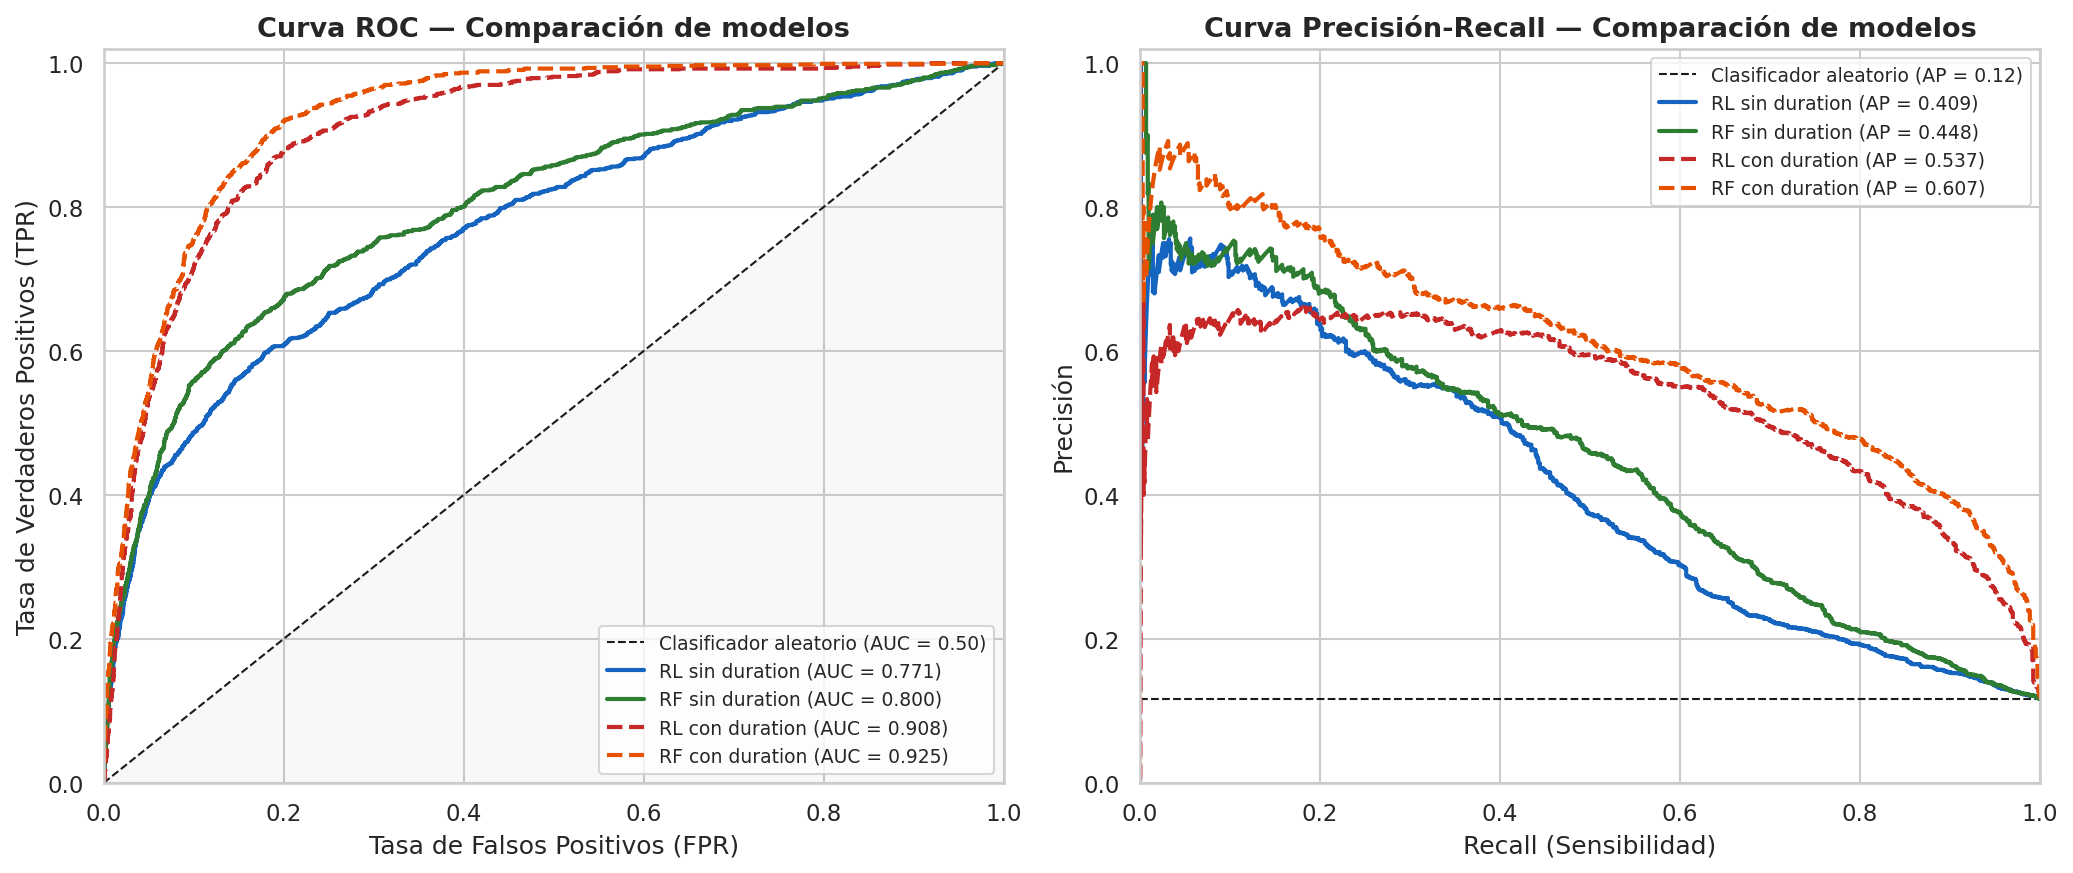
\includegraphics[width=0.95\columnwidth]{curvas_roc_pr.png}
     \caption{Curvas ROC y Precisión-Recall para los cuatro modelos evaluados.}
     \label{fig:curvas}
 \end{figure}

% ============================================================
\section{Conclusiones y Trabajos Futuros}
\label{sec:conclusiones}

\subsection{Conclusiones}

Este trabajo realizó un análisis exploratorio completo del conjunto de datos \textit{Bank Marketing}, revelando patrones estadísticamente relevantes sobre el comportamiento de los clientes bancarios. Las principales conclusiones son:

\begin{itemize}
    \item Las variables numéricas presentan alta asimetría positiva, especialmente \texttt{balance} y \texttt{duration}, con presencia significativa de valores atípicos que deben considerarse en cualquier modelado posterior.
    \item El \textbf{resultado de la campaña anterior} (\texttt{poutcome = success}) es el predictor más potente, con una tasa de suscripción del 64.7\%, seis veces superior a la media.
    \item El \textbf{mes de contacto} tiene un impacto mayor de lo esperado: contactar en marzo, septiembre u octubre duplica o triplica la tasa de éxito frente a mayo, el mes más activo en número de contactos.
    \item El desbalance de clases (11.7\% positivos) es el principal reto del dataset y debe abordarse mediante métricas y técnicas apropiadas como PR-AUC y pesos de clase balanceados.
    \item Los modelos de clasificación confirman que las variables identificadas como relevantes durante la exploración son efectivamente predictivas, validando el valor del análisis exploratorio previo al modelado.
\end{itemize}

\subsection{Trabajos futuros}

\begin{itemize}
    \item Aplicar técnicas de sobremuestreo (SMOTE) para mitigar el desbalance de clases.
    \item Explorar transformaciones de variables (logarítmica, raíz cuadrada) para reducir la asimetría de \texttt{balance} y \texttt{duration}.
    \item Incorporar métodos de explicabilidad (SHAP) para cuantificar la contribución de cada variable a las predicciones individuales.
    \item Evaluar modelos de mayor complejidad como Gradient Boosting (XGBoost, LightGBM).
\end{itemize}

% ============================================================
\section*{Agradecimientos}
Los autores agradecen al repositorio UCI Machine Learning por la disponibilidad pública del conjunto de datos, y al docente Alain Alejo del curso MCD101 por las orientaciones metodológicas recibidas.

% ============================================================
\begin{thebibliography}{9}

\bibitem{tukey1977}
J.\ W.\ Tukey,
\textit{Exploratory Data Analysis}.
Reading, MA: Addison-Wesley, 1977.

\bibitem{moro2014}
S.\ Moro, P.\ Cortez y P.\ Rita,
``A data-driven approach to predict the success of bank telemarketing,''
\textit{Decision Support Systems}, vol.\ 62, pp.\ 22--31, jun.\ 2014.
DOI: \href{https://doi.org/10.1016/j.dss.2014.03.001}{10.1016/j.dss.2014.03.001}

\bibitem{uci_bank}
S.\ Moro, P.\ Rita y P.\ Cortez,
``Bank Marketing,'' UCI Machine Learning Repository, 2012.
DOI: \href{https://doi.org/10.24432/C5K306}{10.24432/C5K306}

\bibitem{crisp2000}
P.\ Chapman \textit{et al.},
``CRISP-DM 1.0: Step-by-step data mining guide,''
SPSS Inc., 2000.
[En línea]. Disponible: \url{https://www.the-modeling-agency.com/crisp-dm.pdf}

\bibitem{ferreira2020}
C.\ Ferreira y A.\ Lopes,
``Predicting bank telemarketing success with gradient boosting methods,''
\textit{Journal of Business Analytics}, vol.\ 3, no.\ 2, pp.\ 98--110, 2020.

\bibitem{bhatt2020}
P.\ Bhatt, A.\ Bhatt y R.\ Singh,
``Handling class imbalance in bank marketing dataset using SMOTE,''
\textit{Proc.\ Int.\ Conf.\ Data Science}, pp.\ 145--152, 2020.

\bibitem{molnar2020}
C.\ Molnar,
\textit{Interpretable Machine Learning: A Guide for Making Black Box Models Explainable},
2.ª ed., 2020.
[En línea]. Disponible: \url{https://christophm.github.io/interpretable-ml-book/}

\end{thebibliography}

\end{document}